\documentclass[tikz,border=8pt]{standalone}
\usepackage{amsmath}
\usetikzlibrary{arrows.meta,decorations.pathreplacing,calc}

\begin{document}
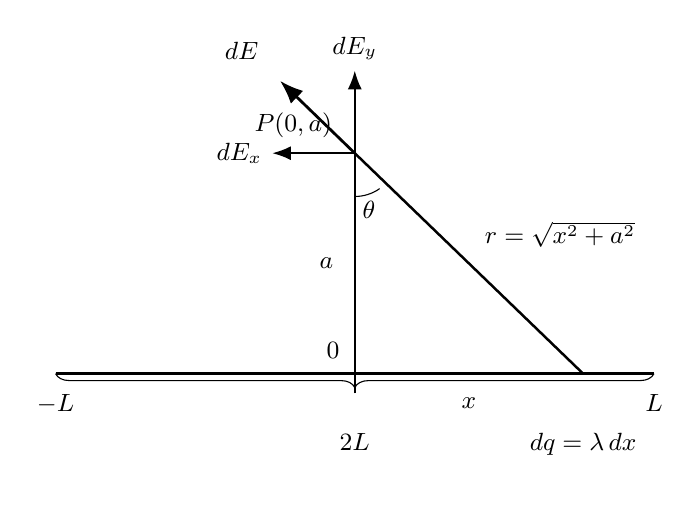
\begin{tikzpicture}[
    line/.style={line width=0.9pt},
    vec/.style={-{Latex[length=3mm]}, line width=1pt},
    thinvec/.style={-{Latex[length=2.4mm]}, line width=0.8pt},
    label/.style={font=\small},
    charge/.style={circle, fill=black, inner sep=1.5pt}
]

% Coordinates
\coordinate (O) at (0,0);
\coordinate (A) at (0,2.8);
\coordinate (Q) at (2.9,0);
\coordinate (L) at (-3.8,0);
\coordinate (R) at (3.8,0);
\coordinate (M1) at (2.65,0);
\coordinate (M2) at (3.15,0);
\coordinate (EyEnd) at ($(A)+(0,1.05)$);
\coordinate (ExEnd) at ($(A)+(-1.05,0)$);

% Rod and axes
\draw[line] (L) -- (R);
\draw[line] (0,-0.25) -- (0,3.25);
\draw[decorate, decoration={brace, amplitude=5pt, mirror}] (L) -- (R)
    node[midway, below=18pt, label] {\(2L\)};

% Observation point and element
\fill[charge] (A);
\node[label] at ($(A)+(-0.78,0.36)$) {\(P(0,a)\)};
\fill[charge] (Q) node[below=4pt, label] {\(dq=\lambda\,dx\)};
\draw[line] (M1) -- (M2);

% Distances
\draw[line] (O) -- (A) node[midway, left=4pt, label] {\(a\)};
\draw[line] (A) -- (Q) node[midway, above right=2pt, label] {\(r=\sqrt{x^2+a^2}\)};
\draw[dashed, line] (O) -- (Q) node[midway, below=5pt, label] {\(x\)};

% Field vector and components at P
\draw[vec] (A) -- ($(A)+(-0.95,0.92)$) node[above left=4pt, label] {\(dE\)};
\draw[thinvec] (A) -- (EyEnd) node[above, label] {\(dE_y\)};
\draw[thinvec] (A) -- (ExEnd) node[left, label] {\(dE_x\)};

% Angle
\draw[thin] ($(A)+(0,-0.55)$) arc[start angle=-90, end angle=-55, radius=0.55];
\node[label] at ($(A)+(0.18,-0.72)$) {\(\theta\)};

% Endpoint labels
\node[label, below=4pt] at (L) {\(-L\)};
\node[label, below=4pt] at (R) {\(L\)};
\node[label, above left=2pt] at (O) {\(0\)};

\end{tikzpicture}
\end{document}
